% !TeX spellcheck = en_GB

\begin{frame}[fragile]{Discrete AdaBoost algorithm}
% stochastic setting
% stochastic gradient boosting framework, when bag.frac < 1
% -> shrinkage added
% -> out-of-bag fraction, on each iteration train a classifier on a different dataset sample, keep the rest as OOB

Discrete AdaBoost with shrinkage and out-of-bag, as an additive model with prediction function $f_m(x)$

{%
\setlength{\interspacetitleruled}{0pt}%
\setlength{\algotitleheightrule}{0pt}%
\begin{algorithm}[H]
\KwIn{$M$, $\set{(x_i,y_i)}_1^N$, $x_i\in\R^p$}
%Initialize observation weights $w_i^{(1)}=1/N$ s.t. $\sum_{i=1}^Nw_i^{(m)}=1$\;
Initialize $f_0(x)=0$\;
\For{$m=1$ \KwTo $M$}{
	Set $w_i^{(m)}=-\frac{\partial L(y,g)}{\partial g}\bigr\rvert_{g=f_m(x)}$ s.t.  $\sum_{i=1}^Nw_i^{(m)}=1$\;
	Fit classifier $G_m(x)$ using $w_i^{(m)}$ with samples from $\pi_m$\;
	Weighted error rate $\text{err}_m=\sum_{i=1}^Nw_i^{(m)}\mathbb{I}(y_i\neq G(x_i))$\;
	Set $\alpha_m=\frac{1}{2}\log\bigl(\frac{1-\text{err}_m}{\text{err}_m}\bigr)$\;
	Update $f_{m}(x)\gets f_{m-1}(x)+\lambda\alpha_mG_m(x)$\;
}
\KwOut{$G(x)=\sign(f_M(x))$}
\end{algorithm}}

\end{frame}

% ------------------------------- %

\begin{frame}{Super Learner algorithm flow diagram}

\begin{figure}
	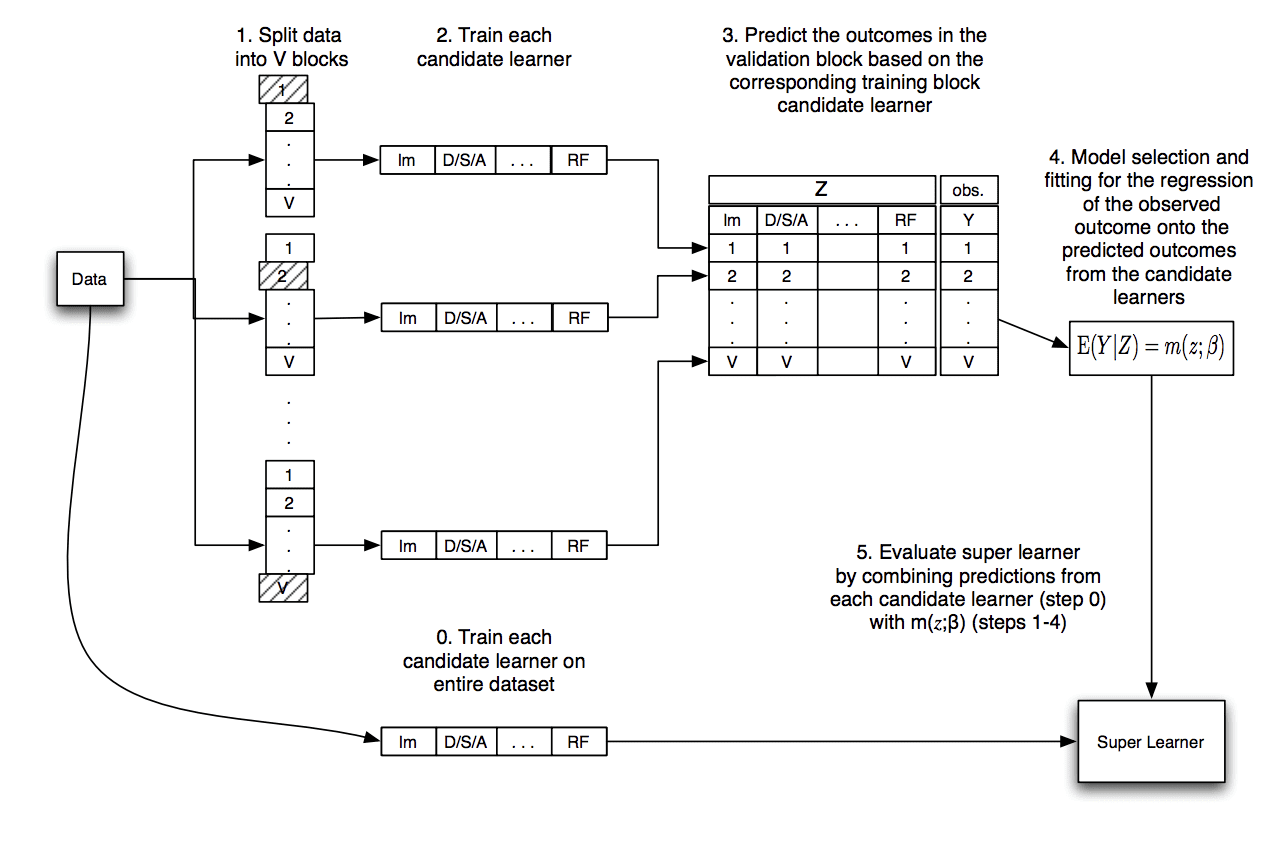
\includegraphics[width=\textwidth]{./Figures/sup-learn.jpg}
\end{figure}

\end{frame}

\begin{frame}[fragile]%{Super learner algorithm}

{%
\setlength{\interspacetitleruled}{0pt}%
\setlength{\algotitleheightrule}{0pt}%
\begin{algorithm}[H]
\KwIn{$\mathcal{D}=\set{(x_i,y_i)}_1^N$, $\mathcal{L}=\set{\phi_k(X)}_{k=1}^K$}
\ForEach{strong learner in $\mathcal{L}$}{%
	Fit $\phi_k$ on $\mathcal{D}$ $\Rightarrow$ $\hat{\phi}_k(\boldsymbol{X})$
	$\rightarrow$ $\hat{\mathcal{L}}=\set{\hat{\phi}_k}_{k=1}^K$\;
}
%Store the fitted library in $\hat{\mathcal{L}}=\set{\hat{\phi}_k(\boldsymbol{X})}_{k=1}^K$\;
\For{$\nu=1,2,\dots,V$}{%
	\ForEach{strong learner in $\mathcal{L}$}{%
		Fit $\phi_k$ on $T(\nu)$, predict $\hat{\phi}_{k,T(\nu)}(X_i\in V(\nu))$\;
	}
}
Stack output in an $N\times K$ matrix
%$Z=\Bigl\{\hat{\phi}_{k,T(\nu)}\bigl(X_{V(\nu)}\bigr),\,\nu=1,2,\dots,V,\,k=1,2,\dots,K\Bigr\}$\;
$Z=\bigl\{\hat{\phi}_{k,T(\nu)}\bigl(X_{V(\nu)}\bigr)\bigr\}$\;
Propose a family of weighted combinations\vspace{-1em}
\[
m(z\rvert\alpha)=\sum_{k=1}^K\alpha_k\hat{\phi}_{k,T(\nu)}\bigl(\boldsymbol{X}_{V(\nu)}\bigr)
\rightarrow
\hat{\alpha}=\argmin_\alpha\sum_{i=1}^NL(Y_i,m(z_i\rvert\alpha))
\vspace*{-1em}\]
of size $N$ s.t. $\alpha_k\geq0$, $\sum_k\alpha_k=1$ and minimizes $\sum_k\alpha_k\hat{\phi}_k$\;
Combine $\hat{\alpha}$ with the library $\hat{\mathcal{L}}$ $\rightarrow$ 
$\hat{\phi}_{\text{SL}}(\boldsymbol{X})=\sum_{k=1}^K\hat{\alpha}_k\hat{\phi}_k(\boldsymbol{X})$\;
\KwOut{$\hat{\phi}_{\text{SL}}$}
\end{algorithm}}

\end{frame}
